% aliveKat, presentation to IFO-SIM, Saturday 19th of Dec
\documentclass[12pt]{beamer}
\mode<presentation> {
\usetheme{Madrid}
\setbeamertemplate{navigation symbols}{}
}

\usepackage[utf8]{inputenc}
\usepackage{amsmath, amssymb, amsthm}
\usepackage{amsfonts}
\usepackage{graphicx}
\usepackage{float}  % bunch of formatting stuff
\usepackage[center]{caption}
\usepackage{hyperref}
\usepackage{mathtools}

\usepackage{subfig}
\usepackage{comment}
% \usepackage{siunitx}

\usepackage{xcolor}

% \usepackage{booktabs} % toprule, \midrule and \bottomrule in tables
% \newcommand\hmmax{0}  % stop the 'too many math scripts' error
% \newcommand\bmmax{0}

% \usepackage{bibentry}

\newcommand{\code}[1]{\texttt{#1}}


%TITLE PAGE
\title[Verification of the \code{nle}]{Verification of the newly-added non-linear element in Finesse for optical modelling of advanced gravitational-wave detector configurations}

\author[James W. Gardner et al.]{James~W.~Gardner, Vaishali~B.~Adya, Daniel~Töyrä, David~McClelland}
\institute[ANU-CGA]{Centre for Gravitational Astrophysics (CGA), ANU}
\date{\today}

\begin{document}

{
  \usebackgroundtemplate{\includegraphics[width=\paperwidth]{figures/title_slide_with_logos.pdf}}
  \begin{frame}
  % \titlepage
  \end{frame}
}

%%%%%%%%%%%%%%%%%%%%%%%%%%%%%%%%%%%%%%%%%%

\begin{frame}{Motivation - HF sensitivity}
% GW detectors and neutron stars as example of HF source
\begin{figure}
\includegraphics<1>[height=\textwidth,angle=-90]{figures/gwo_ifos-pictures.pdf}
\caption*{LIGO-Hanford, LIGO-Livingston, VIRGO, KAGRA}
\end{figure}
% quantum noise at HF
\end{frame}

% quantum noise in phase quadrature
\begin{frame}{aLIGO with long SRC and internal squeezing}
\begin{columns}
\column{0.5\textwidth}
\centering
\includegraphics<1>[height=.7\textheight]{figures/aLIGO_internal_squeezing.pdf}

\column{0.5\textwidth}
{\centering
\includegraphics<1>[width=\textwidth]{figures/sqz_aLIGO_analytics_quantum_noise_budget-labelled.pdf}
}
{\footnotesize \vspace{-0.1cm} Such a configuration may\!~\footnote{\tiny{Mikhail Korobko, Yiqiu Ma, Yanbei Chen, and Roman Schnabel.\\ Quantum expander for gravitational-wave observatories. \emph{Light: Science\\ \& Applications}, 8(1), Dec 2019.}}\!~\footnote{\tiny{V B Adya, M J Yap, D Töyrä, et al. Quantum enhanced kHz \\gravitational wave detector with internal squeezing. \emph{Classical and \\Quantum Gravity}, 37(7):07LT02, Mar 2020.}} improve the HF QN limited:}
\begin{itemize}
    \scriptsize
\item peak sensitivity
\item broadband sensitivity\vspace{-0.2cm}
\end{itemize}

\end{columns}
% Mikhail Korobko, Yiqiu Ma, Yanbei Chen, and Roman\\ Schnabel. Quantum expander for gravitational-wave\\ observatories. \emph{Light: Science \& Applications}, 8(1), Dec 2019.
% \vspace{-.5cm}
% \includegraphics<2>[height=.8\textheight]{figures/aLIGO_transfer_fns_and_sensitivity_comparison.pdf}
\end{frame}

\begin{frame}{Project timeline}
% \begin{block}{Test the new \code{nle} component in Finesse}
\begin{itemize}
\item we want to see HF GW sources
\item proposed configuration may improve HF QN limited sensitivity
\item we need the \code{nle} in Finesse to model the configuration
\item equations provided by Daniel~Töyrä
% sqz matrix equations
\item implementation by Daniel~Brown~\footnote{available at {\color{blue}\url{https://git.ligo.org/finesse/finesse/-/tree/nle}}}
\item testing by James~Gardner~\footnote{available at {\color{blue}\url{https://github.com/daccordeon/aliveKat}}}$\longleftarrow$(this talk!)
    \begin{itemize}
    \item does it work? \footnote{spoiler: likely yes but it is a work-in-progress}
    \end{itemize}
% \item what’s Finesse?
\end{itemize}
% If successful, then allows us an efficient means to test configurations
% \end{block}
\end{frame}

% freq. domain optical modelling, used in GW field and for optical cavities
% Finesse can do (cool stuff) ...
\begin{frame}{Finesse}
% \only<2-|handout:0>{\stepcounter{framenumber}}
\begin{itemize}
\item<1> frequency domain optical modelling 
% \item e.g.\ can handle beam geometry, noise coupling, higher order modes
\item<1> can model some realistic effects
\item<1> used for GW detector proposals and outside GW research
\end{itemize}
\begin{figure}
    \captionsetup[subfigure]{labelformat=empty}
    \centering 
    \subfloat[\centering]{{\includegraphics<1>[width=0.2\textwidth]{figures/finesse_horse.png}}}%    
    \qquad
    \subfloat[\centering]{{\includegraphics<1>[width=0.5\textwidth]{figures/pykat_cat_and_pie.png}}}%
\end{figure}
\only{
\vfill
{\color{blue}\url{http://www.gwoptics.org/finesse/}}
}<1>
% \only{
% \vspace{-4cm}
% }<2>
\end{frame}

\begin{frame}{Non-linear element matrix}
% The matrix for the non-linear crystal in the two-photon formalism is
Two-photon formalism/quadrature picture (analytics)
{\footnotesize
\begin{align}
\mathbf{N} &\equiv \mathbf{N}(r, \phi) = \begin{bmatrix} \cosh(r) + \sinh(r) \cos(2\phi) & \sinh(r) \sin(2\phi) \\ 
                                            \sinh(r) \sin(2\phi) & \cosh(r) - \sinh(r) \cos(2\phi)
                                            \end{bmatrix}
\end{align}
}
\vspace{-0.5cm}
\begin{align}
\begin{bmatrix}
\hat{b}_{1} \\
\hat{b}_{2}  
\end{bmatrix} = \mathbf{N} \begin{bmatrix}
\hat{a}_{1} \\
\hat{a}_{2}
\end{bmatrix}
\end{align}
% e.g. for $\vec{u}$ the incident field and $\vec{v}$ the transmitted field expressed as quadrature vectors
% \begin{align}
% \vec{v} = \mathbf{N}\, \vec{u}
% \end{align}
% Alternatively, the matrix going into Finesse is in the sideband picture
One-photon formalism/sideband picture (Finesse)
{\footnotesize
\begin{align}
\mathbf{N} &\equiv \mathbf{N}(r, \phi) = \begin{bmatrix} \cosh(r) & \text{e}^{2i\phi} \sinh(r) \\ 
                              \text{e}^{-2i\phi} \sinh(r) & \cosh(r)
                     \end{bmatrix}
\end{align}
}
\vspace{-0.5cm}
\begin{align}
\begin{bmatrix}
\hat{b}_{\omega_0 + \Omega} \\
\hat{b}^\dagger_{\omega_0 - \Omega}  
\end{bmatrix} = \mathbf{N} \begin{bmatrix}
\hat{a}_{\omega_0 + \Omega} \\
\hat{a}^\dagger_{\omega_0 - \Omega}
\end{bmatrix}
\end{align}

\end{frame}

\begin{frame}{Finesse squeezer conventions}
\begin{columns}
\column{0.5\textwidth}
% \captionsetup[subfigure]{labelformat=empty}
\centering 
% \subfloat[\centering]{{\includegraphics<2>[width=0.4\textwidth]{figures/testing_Finesse_squeezers-sq.pdf}}}%
% \qquad
% \subfloat[\centering]{{\includegraphics<2>[width=0.4\textwidth]{figures/testing_Finesse_squeezers-nle.pdf}}}%
\includegraphics<1>[width=\textwidth]{figures/testing_Finesse_squeezers_comparison.pdf}

\column{0.5\textwidth}
\tiny
\code{nle}:
    \begin{itemize}
    \item connects two nodes (can be internal),
    % \item produces $20 \log_{10}(e^r)$ worth of squeezing given input r,
    \item internally converts input $x$ to $r_\code{nle} = \frac{x}{10} \log(10)$,
    \item squeezes (noise, signal, but not carrier) fields in both directions,
    \item \code{nle name r\_sqz angle\_sqz node\_1 node\_2} 
    \end{itemize}
\code{sq}:
    \begin{itemize}
    \item connects to one node (for external input),
    % \item produces $10 \log_{10}(e^r)$ worth of squeezing given input r,
    \item internally converts input $x$ to $r_\code{sq} = \frac{x}{20} \log(10)$,
    \item \code{sq name f r\_sqz angle\_sqz node}
    \end{itemize}
\end{columns}
\end{frame}

% \begin{frame}{Our goal}
% \begin{block}{Test the new \code{nle} component in Finesse}
% If successful, then allows us an efficient means to test configurations
% \end{block}
% \end{frame}

%%%%%%%%%%%%%%%%%%%%%%%%%%%%%%%%%%%%%%%%%%

\begin{frame}{Squeezed cavity}
\centering
\includegraphics<1>[height=0.8\textwidth, angle=-90]{figures/squeezed_cavity.pdf}
\end{frame}

\begin{frame}{Squeezed cavity - analytics\footnote{\tiny See the complete derivation at {\color{blue}\url{https://github.com/daccordeon/aliveKat}}}}
\tiny
% (two-photon formalism)
In the frequency domain, the vacuum noise incident on the cavity can be expressed in the two-photon formalism/quadrature picture as
\begin{align}
\vec{a}(\Omega) = \begin{bmatrix}
    \hat{a}_1(\Omega) \\
    \hat{a}_2(\Omega)
\end{bmatrix}
\end{align}

The field reflected off the cavity is
\begin{align}
\vec{b}(\Omega) = \begin{bmatrix}
    \hat{b}_1(\Omega) \\
    \hat{b}_2(\Omega)
\end{bmatrix} = \mathbf{M}\, \vec{a}(\Omega)
\end{align}

where the matrix describing the reflection off the cavity is
\begin{align}
\mathbf{M} &= -\mathbf{R_1} + \mathbf{T_1} ( \mathbf{I} - \mathbf{N}\, \mathbf{P}\, \mathbf{R_2}\, \mathbf{P}\, \mathbf{N}\, \mathbf{R_1} )^{-1} \mathbf{N}\, \mathbf{P}\, \mathbf{R_2}\, \mathbf{P}\, \mathbf{N}\, \mathbf{T_1} %\\
% \mathbf{M} &= -\mathbf{R} + \mathbf{T} ( \mathbf{I} - \mathbf{N}\, \mathbf{S}\, \mathbf{N}\, \mathbf{R} )^{-1} \mathbf{N}\, \mathbf{S}\, \mathbf{N}\, \mathbf{T} \\
% \mathbf{R} &- \text{Reflection off input mirror} \\
% \mathbf{T} &- \text{Transmission through input mirror} \\
% \mathbf{S} &- \text{Roundtrip propagation} \\
% \mathbf{I} &- \text{Identity matrix} \\
\end{align}

where $\mathbf{I}$ is the identity matrix, $\mathbf{R_n}\, (\mathbf{T_n})$ is the reflection (transmission) matrix for the nth mirror, $\mathbf{P}$ is propagation across the cavity interior, and the matrix for the non-linear crystal is
\begin{align}
\mathbf{N} &\equiv \mathbf{N}(r, \phi) = \begin{bmatrix} \cosh(r) + \sinh(r) \cos(2\phi) & \sinh(r) \sin(2\phi) \\ 
                                            \sinh(r) \sin(2\phi) & \cosh(r) - \sinh(r) \cos(2\phi)
                                            \end{bmatrix}
\end{align}

The operator for the homodyne readout power-fluctuations is
\begin{align}
\hat{P}(\Omega) =  A_1 \big(\hat{b}_1(\Omega) + \hat{b}_1^\dagger(\Omega) \big) + A_2 \big(\hat{b}_2(\Omega) + \hat{b}_2^\dagger(\Omega) \big)
\end{align}

where $A_1 = \sqrt{P_0}\cos(\theta)$ and $A_2 = \sqrt{P_0}\sin(\theta)$, $P_0$ is the power of the local oscillator, and $\theta$ is the phase of the local oscillator. The power spectral density (PSD) and amplitude spectral density (ASD) of the quantum noise become
\begin{align}
\text{PSD} &= \langle0|\, \hat{P}(\Omega) \hat{P}^\dagger(\Omega) \,| 0\rangle = 
2 P_0 \hbar \omega_0 \,[\,\cos(\theta) \; \sin(\theta)\,]\, \mathbf{M} \,\mathbf{M}^\dagger \begin{bmatrix} \cos(\theta) \\ \sin(\theta) \end{bmatrix} \\
\text{ASD} &= \sqrt{\text{PSD}}
\end{align}


\vspace{-.5cm}
\end{frame}

% show method!
\begin{frame}{Squeezed cavity - squeezer response}
% \only<2-|handout:0>{\stepcounter{framenumber}}
\centering
% \qquad
% \begin{columns}
% \column{0.5\textwidth}
% \includegraphics<2>[width=\textwidth]{figures/not_main_PSD_vs_r.pdf}
% \column{0.5\textwidth}
% \includegraphics<2>[width=\textwidth]{figures/pykat_relative_qhd_vs_r.pdf}
% \end{columns}
\includegraphics<1>[width=0.8\textwidth]{figures/squeezed_cavity_relative_qhd_vs_r_comparison_2.pdf}
\end{frame}

\begin{frame}{Squeezed cavity - conclusions}
\begin{block}{Initial verification for the \code{nle}}
\begin{itemize}
\item Finesse agrees with analytics for 
    \begin{itemize}
    \item \code{nle} in isolation
    % \item empty cavity
    \item \code{nle} in cavity
    \end{itemize}
% \item We also re-derived the analytics another three different ways which all agree with each other
\end{itemize}
\end{block}
% \begin{alertblock}{Limitations}
% \begin{itemize}
% \item We have only considered plane waves, e.g.\ we do not know the interaction with \code{maxtem}
% \item We have only shown relative scales, to compare the exact values for the ASD we are still chasing some factors of $2$ and $c$.
% \end{itemize}
% \end{alertblock}
\end{frame}

%%%%%%%%%%%%%%%%%%%%%%%%%%%%%%%%%%%%%%%%%%

% match powers, check tunings, then compare sensitivities
\begin{frame}{aLIGO with long SRC and internal squeezing}
\only<2-|handout:0>{\stepcounter{framenumber}}
\centering 
\begin{columns}
\column{0.5\textwidth}
\includegraphics<1>[width=\textwidth]{figures/aLIGO_internal_squeezing.pdf}
\column{0.5\textwidth}
\includegraphics<1>[width=\textwidth]{figures/aLIGO_as_coupled_cavities.pdf}
\end{columns}
\vspace{-.5cm}
\includegraphics<2>[height=.88\textheight]{figures/aLIGO_transfer_fns_and_sensitivity_comparison.pdf}
\includegraphics<3>[height=0.8\textwidth, angle=-90]{figures/sqz_aLIGO_analytics_v_simulation_with_fractional_errors.pdf}        
\end{frame}

% rewrite this
\begin{frame}{Conclusions}
\begin{block}{Work-in-progress verification of the \code{nle}}
\begin{itemize}
\item Works in isolation 
\item Agrees with analytics for the squeezed cavity
\item Agrees with analytics for aLIGO up to a $5\%$ fractional error
\item Need to be aware of input conventions used by the \code{nle}
\end{itemize}
\end{block}

\begin{alertblock}{Limitations}
\begin{itemize}
\item We have only considered plane waves, e.g.\ we do not know the interaction with \code{maxtem}
\item We have only shown relative scales, to compare the exact values for the ASD we are still chasing some factors of $2$ and $c$.
\end{itemize}
\end{alertblock}
\end{frame}

\begin{frame}{Future work}
\begin{itemize}
\item Finish verification
\item Determine reason for deviation from analytics
\item Test signal sidebands
\item Optimisation for HF sensitivity
\end{itemize}
% \begin{block}{Optimisation for HF sensitivity}
% % Can use Finesse to find the optimum configuration
% \end{block}
\begin{block}{Modelling exotic configurations}
\begin{itemize}
\item Detuned long SRC
\item Non-degenerate squeezing
\end{itemize}
\end{block}
\end{frame}


%%%%%%%% repete primeiro slide %%%%%%%%
\begin{frame}
\titlepage 
\end{frame}

\begin{frame}[noframenumbering]{Squeezed cavity - frequency response}
% \only<2-|handout:0>{\stepcounter{framenumber}}
\centering
% \includegraphics<1>[width=0.9\textwidth]{figures/not_main_PSD_vs_freq.pdf}%
% % \vspace{-.1cm}
% \includegraphics<2>[width=0.8\textwidth]{figures/pykat_relative_qhd_vs_freq.pdf}%
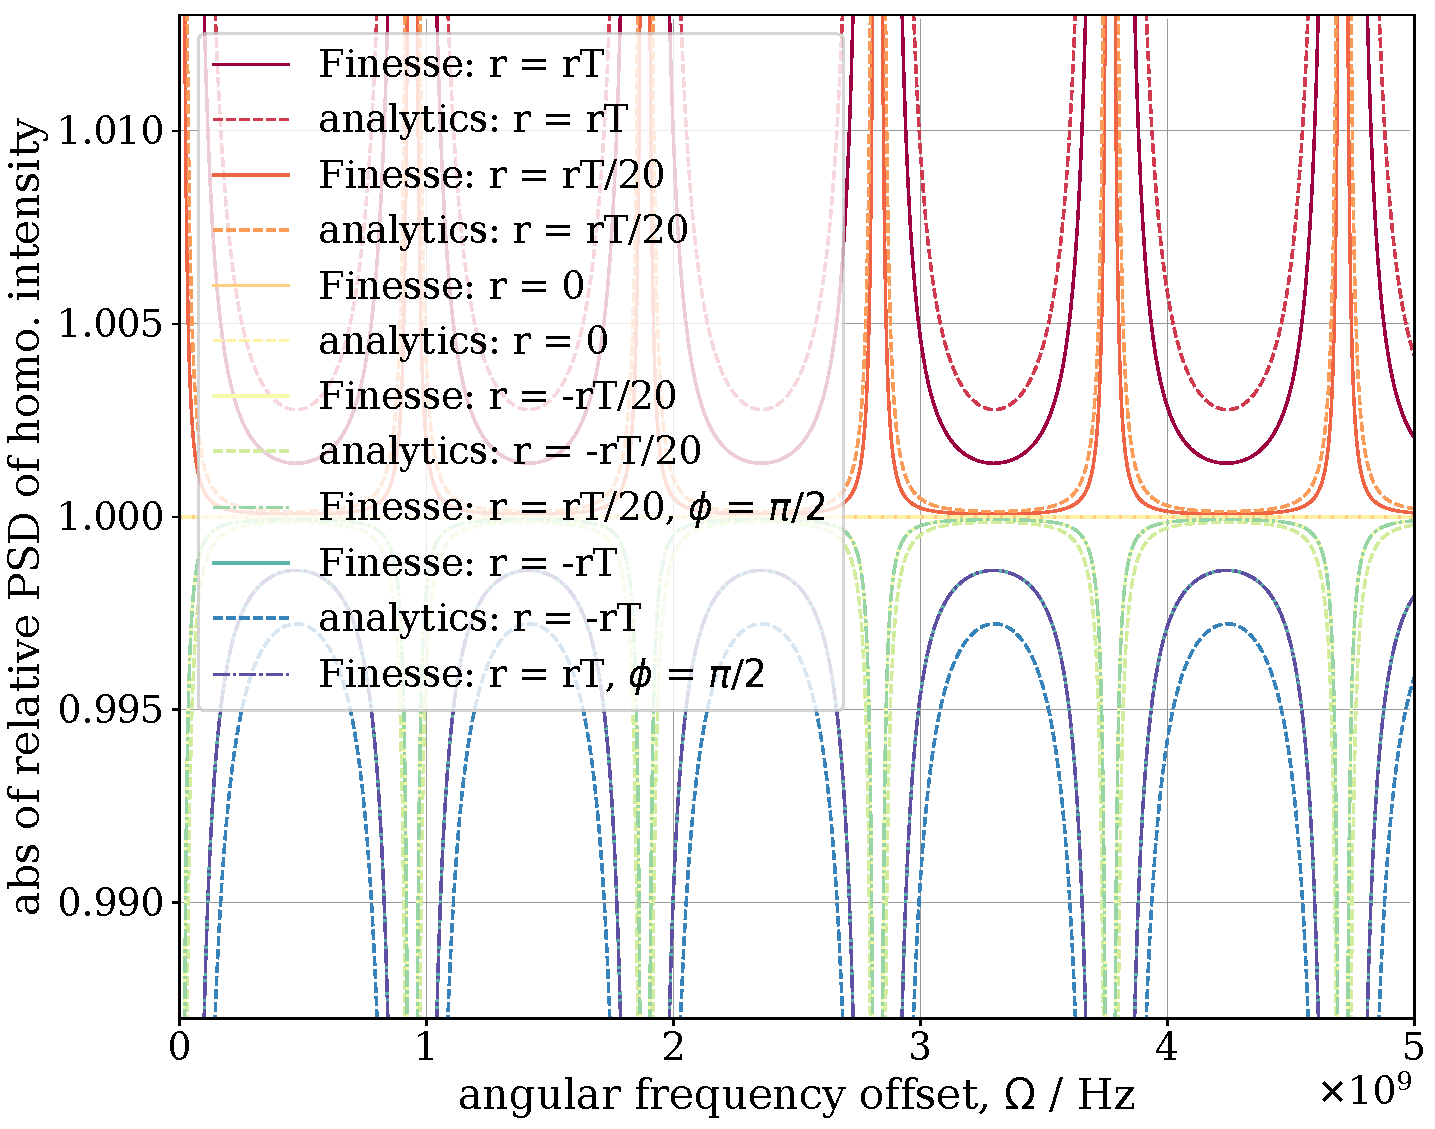
\includegraphics[width=0.8\textwidth]{figures/squeezed_cavity_relative_qhd_vs_freq_comparison.pdf}
\end{frame}

% \begin{frame}{Example of optimisation}
% \centering 
% \includegraphics<1>[height=0.85\textheight]{figures/aLIGO_optimum_sensitivity_comparison.pdf}
% \end{frame}

% \begin{frame}{wrong - Squeezed cavity analytics}
% % {\big wrong!}
% \begin{columns}
% \column{0.5\textwidth}
% $$S_\mathrm{HomI}(\Omega) = \frac{A_0^2 \left( g_1(\Omega)^2 + g_2(\Omega)^2 \right)}{g_3(\Omega)^2}$$
% \column{0.5\textwidth}
% \tiny
% \begin{align*}
% g_1 &= -\cosh ^2(r) e^{\frac{2 i L \Omega }{c}} (\cos (\theta ) \left(2 r_1^2+t_1^2\right) \cos (2 \psi )\\
%     &+t_1^2 \sin (\theta ) \sin (2 \psi )) \\
%     &-\cos (\theta ) \sinh ^2(r) \left(2 r_1^2+t_1^2\right) e^{\frac{2 i L \Omega
%     }{c}}\\
%     &-t_1^2 \cos (\theta ) \sinh (2 r) \cos (\psi ) \cos (2 \phi ) e^{\frac{2 i L \Omega }{c}}\\
%     &-t_1^2 \sin (\theta )
%     \sinh (2 r) \cos (\psi ) \sin (2 \phi ) e^{\frac{2 i L \Omega }{c}}\\
%     &+r_1^3 \cos (\theta ) e^{\frac{4 i L \Omega
%     }{c}}+r_1 t_1^2 \cos (\theta ) e^{\frac{4 i L \Omega }{c}}+r_1 \cos (\theta ) \\
% g_2 &= \cosh ^2(r) e^{\frac{2 i L \Omega }{c}} (t_1^2 \cos (\theta ) \sin (2 \psi )\\
%     &-\sin (\theta ) \left(2 r_1^2+t_1^2\right) \cos (2 \psi ))\\
%     &+\sin (\theta ) \left(-\sinh ^2(r) (2 r_1^2+t_1^2\right)
%     e^{\frac{2 i L \Omega }{c}}\\
%     &+t_1^2 \sinh (2 r) \cos (\psi ) \cos (2 \phi ) e^{\frac{2 i L \Omega }{c}}\\
%     &+r_1^3 e^{\frac{4 i L \Omega }{c}}+r_1 t_1^2 e^{\frac{4 i L \Omega }{c}}+r_1)\\
%     &-4 t_1^2 \cos (\theta ) \sinh (r) \cosh (r) \cos (\psi ) \sin (\phi ) \cos (\phi ) e^{\frac{2 i L \Omega }{c}} \\
% g_3 &= 1 + r_1^2 e^{\frac{4 i L \Omega}{c}} - 2 e^{\frac{2 i L \Omega}{c}} \sinh(r)^2 \\
%     &- 2 e^{\frac{2 i L \Omega}{c}} r_1 \cos(2 \psi) \cosh(r)^2 
% \end{align*}
% \normalsize
% \end{columns}
% \end{frame}

% \begin{frame}{Finesse code example}
% \centering 
% \includegraphics<1>[height=0.85\textheight]{figures/finesse_code_example.png}
% \end{frame}

\end{document}
